
\documentclass[12pt]{article}

\usepackage[utf8]{inputenc}
\usepackage[greek, english]{babel}

% Packages

\usepackage{alphabeta}
\usepackage{amsmath}
\usepackage{amsthm}
\usepackage{caption}
\usepackage{color}
\usepackage{fullpage}
\usepackage{graphicx}
\usepackage{latexsym}
\usepackage{listings}
\usepackage{pxfonts}
\usepackage{stackrel}
\usepackage{titlesec}
\usepackage{subfig}
\usepackage{tikz}
\usepackage{float}
\usepackage{hyperref}

% Commands
\newcommand{\R}{\mathbb{R}}
\newcommand{\N}{\mathbb{N}}
\newcommand{\norm}[1]{\left\lVert#1\right\rVert}
\newcommand{\margin}{\hspace{4pt}}
\newcommand{\centered}[1]{\begin{align*}#1\end{align*}}
\newcommand{\code}[2]{\lstinputlisting[caption={#2}]{#1}}

% Environments
\newenvironment{rcases}
	{\left.\begin{aligned}}
	{\end{aligned}\right\rbrace}

\newenvironment{matlab}
	{\begin{figure}[H]\centering\captionsetup{justification=centering}}
	{\end{figure}}

% Python Syntax Highlighting
\definecolor{string_color}{RGB}{0, 161, 13}
\definecolor{comment_color}{RGB}{46, 46, 46}
\definecolor{keyword_color}{RGB}{0, 112, 191}
\definecolor{background_color}{RGB}{250, 250, 250}

\lstset{
    framesep=10pt,
    xleftmargin=10pt,
    xrightmargin=10pt,
    language=Python,
    captionpos=b,
    numbers=right,
    numberstyle=\small\ttfamily,
    frame=lines,
    showspaces=false,
    showtabs=false,
    breaklines=true,
    showstringspaces=false,
    breakatwhitespace=true,
    commentstyle=\color{comment_color}\textit,
    keywordstyle=\bfseries\color{keyword_color}\textbf,
    stringstyle=\color{string_color}\textit,
    morekeywords={self, lambda, __init__, __del__, __name__, for, in, not, and, or, :},
    basicstyle=\small\ttfamily,
    tabsize=4,
    keepspaces=true,
    columns=flexible,
    backgroundcolor=\color{background_color}
}

\hypersetup{
    colorlinks=true,
    linkcolor=blue,
    filecolor=magenta,
    urlcolor=cyan,
}

% Lengths
\setlength{\parindent}{0in}
\setlength{\oddsidemargin}{0in}
\setlength{\textwidth}{6.5in}
\setlength{\textheight}{10in}
\setlength{\topmargin}{-1.0in}
\setlength{\headheight}{18pt}

\titlespacing*{\subsection}
{0pt}{5.5ex plus 1ex minus .2ex}{4.3ex plus .2ex}

\title{\huge Examples of Linear Programming Problems\\Pattern Classification}
\author{Σιώρος Βασίλειος\\Ανδρινοπούλου Χριστίνα}
\date{Νοέμβριος 2019}

\begin{document}

\maketitle

\pagenumbering{gobble}

\pagebreak

\section{Feature Vectors}

Έστω \textbf{m} αντικείμενα, τα οποία επιθυμούμε να ταξινομήσουμε σε δύο διακριτές ομάδες,
με κάθε αντικείμενο να ανήκει αυστηρά σε μία μόνο ομάδα. \\

Παραδείγματος χάριν \textbf{φυτά}, που επιθυμούμε να διαχωρίσουμε σε \textbf{εσπεριδοειδή} και \textbf{μη}.\\

Θεωρούμε πως τα αντικείμενα αυτά περιγράφονται επαρκώς από \textbf{n} το πλήθος χαρακτηριστικά. \\

Στην περίπτωση της ταξινόμησης φυτών, σε εσπεριδοειδή και μη, τα χαρακτηριστικά αυτά θα μπορούσαν
να είναι το \textbf{ύψος} του δέντρου, αν είναι \textbf{φυλλοβόλο} ή όχι, δηλαδή αν ρίχνει τα φύλλα του το χειμώνα και σε τι \textbf{κλίμα} ευδοκιμεί.

Μπορούμε λοιπόν, να αναπαραστίσουμε κάθε αντικείμενο με ένα \textbf{n}-διάστατο διάνυσμα. \\

Παραδείγματος χάριν, έστω ένα στιγμιότυπο \(x\) της κλάσης των εσπεριδοειδών με τα εξής \textbf{3} χαρακτηριστικά

\begin{align*}
    &\text{Ύψος : } \textit{8m} \\
    &\text{Φυλλοβόλο : } \textit{Όχι} \\
    &\text{Κλίμα : } \textit{Τροπικό} \vee \textit{Υποτροπικό} \vee \textit{Eύκρατο}
\end{align*}

τότε, το παραπάνω αντικείμενο μπορεί να αναπαρασταθεί από το \textbf{3}-διάστατο διάνυσμα

\centered{x^* = [\textit{8m}, \margin \textit{Όχι}, \margin \textit{Τροπικό} \vee \textit{Υποτροπικό} \vee \textit{Eύκρατο}]}

Είναι προφανές από το προηγούμενο παράδειγμα, ότι τα χαρακτηριστικά των αντικειμένων μπορεί να είναι μη αριθμητικά.
Ωστόσο, υπάρχουν μέθοδοι μετατροπής τους σε αριθμητικά κι ως εκ τούτου, το παραπάνω διάνυσμα μπορεί εύκολα να απεικονιστεί στον \( \R^{3} \).
Λοιπόν, θα εστιάσουμε στην περίπτωση των αριθμητικών χαρακτηριστικών. \\

Εις το εξής, οι όροι αντικείμενο και διάνυσμα θα χρησιμοποιούνται ισοδύναμα. \\

\pagebreak

\section{Linear Separability}

Δεδομένης της προηγουμένως ορισθείσας αναπαράστασης αντικειμένων, θεωρούμε τα σύνολα

\begin{align*}
    K & = \{K_{1}, K_{2}, \dotsc , K_{l_k}\} & \text{ όπου }  K_i \in \R^{n} & \margin \forall i \in \lbrack 1, \dotsc l_k \rbrack \\
    N & = \{N_{1}, N_{2}, \dotsc , N_{l_n}\} & \text{ όπου }  N_i \in \R^{n} & \margin \forall i \in \lbrack 1, \dotsc l_n \rbrack
\end{align*}

Γνωρίζουμε ότι, ένα υπερεπίπεδο διαχωρίζει ένα αφινικό χώρο σε δύο ημιχώρους. \\

Τα σύνολα \(K\) και \(N\) χαρακτηρίζονται \textbf{γραμμικά} διαχωρίσιμα,
αν υπάρχει υπερεπίπεδο, τέτοιο ώστε τα αντικείμενα,
που ανήκουν στο σύνολο Κ να εντοπίζονται στον έναν ημιχώρο και τα αντικείμενα,
που ανήκουν στο σύνολο N στον άλλον ημιχώρο. \\

Πιο τυπικά θα λέγαμε ότι τα σύνολα Κ και N χαρακτηρίζονται \textbf{γραμμικά} διαχωρίσιμα,
αν υπάρχουν \( a \in \R^{n} \) και \( b \in \R \), τέτοια ώστε

\begin{align*}
    K & \subseteq \{ x \in \R^{n} : a^{T} \cdot x \geq b \} \\
    N & \subseteq \{ x \in \R^{n} : a^{T} \cdot x < b\}
\end{align*}

\begin{figure}[hp]
    \centering
    \subfloat[Γραμμικά διαχωρίσιμα σύνολα]{{\includegraphics[width=7.5cm]{figures/linearly_separable}}}
    \qquad
    \subfloat[Μη γραμμικά διαχωρίσιμα σύνολα]{{\includegraphics[width=7.5cm]{figures/not_linearly_separable}}}
    \caption{Παράδειγμα γραμμικής διαχωρισιμότητας στον \( \R^2 \)}
\end{figure}

\pagebreak

\section{Pattern Classification via Linear Programming}

\subsection{Pattern Classification}

Mπορούμε να εκφράσουμε τη γραμμική διαχωρισιμότητα ως εξής: \\

Έστω τα δύο σύνολα αντικειμένων: 

\begin{align*}
K & = \{K_{1}, K_{2}, \dotsc , K_{l_k}\} & \text{ όπου }  K_i \in \R^{n} & \margin \forall i \in \lbrack 1, \dotsc l_k \rbrack \\
N & = \{N_{1}, N_{2}, \dotsc , N_{l_n}\} & \text{ όπου }  N_i \in \R^{n} & \margin \forall i \in \lbrack 1, \dotsc l_n \rbrack
\end{align*}

Τα \(K\) και \(N\) είναι γραμμικά διαχωρίσιμα αν και μόνο αν υπάρχει \(a \in \R^{n}\) και \(b \in \R\) τέτοια ώστε \(a^{T} \cdot K_{i} -b \geq 1\) και \(a^{T} \cdot N_{j} - b \leq -1\) \(\forall i \in \{1,...,l_{k}\}\) και \(\forall j \in \{1,...,l_{n}\}\). \\

Για να αποδείξουμε τον παραπάνω ισχυρισμό, πρέπει να αποδείξουμε και τις δύο κατευθύνσεις: \\

\( \bullet \) Αν υπάρχει \(a \in \R^{n}\) και \(b \in \R\) τέτοια ώστε \(a^{T} \cdot K_{i} -b \geq 1\) και \(a^{T} \cdot N_{j} - b \leq -1\) \(\forall i \in \{1,...,l_{k}\}\) και \(\forall j \in \{1,...,l_{n}\}\), τότε τα \(K\) και \(N\) είναι γραμμικά διαχωρίσιμα \\

Όπως προαναφέρθηκε, τα \(K\) και \(N\) είναι γραμμικά διαχωρίσιμα όταν υπάρχουν \( a \in \R^{n} \) και \( b \in \R \), τέτοια ώστε

\begin{align*}
K & \subseteq \{ x \in \R^{n} : a^{T} \cdot x \geq b \} \\
N & \subseteq \{ x \in \R^{n} : a^{T} \cdot x < b\}
\end{align*}

Άρα, προφανώς τα \(K\) και \(N\) θα είναι γραμμικά διαχωρίσιμα και όταν: \\

\begin{align*}
K & \subseteq \{ x \in \R^{n} : a^{T} \cdot x \geq b + 1 \} \\
N & \subseteq \{ x \in \R^{n} : a^{T} \cdot x < b - 1\}
\end{align*}

\( \bullet \)  Αν τα \(K\) και \(N\) είναι γραμμικά διαχωρίσιμα, τότε υπάρχει \(a \in \R^{n}\) και \(b \in \R\) τέτοια ώστε \(a^{T} \cdot K_{i} -b \geq 1\) και \(a^{T} \cdot N_{j} - b \leq -1\) \(\forall i \in \{1,...,l_{k}\}\) και \(\forall j \in \{1,...,l_{n}\}\). \\

Αφού τα \(K\) και \(N\) είναι γραμμικά διαχωρίσιμα, υπάρχουν \( c \in \R^{n} \) και \( b \in \R \), τέτοια ώστε \(c^{T} \cdot x \geq b \) για \(x \in K\) και \(c^{T} \cdot x < b \) για \(x \in Ν\). \\

Ορίζουμε \textit{m} (εκ του margin) ως:

\centered{ m = \min_{x \in K} c^{T} \cdot x - \max_{x \in N} c^{T} \cdot x }

Επειδή ισχύει ότι: \\

\centered{a = \frac{2}{m} \cdot c}
\centered{b = \frac{1}{p} \cdot \left( \min_{x \in K} c^{T} \cdot x + \max_{x \in N} c^{T} \cdot x \right)}

Για το \(\max_{x \in N} a^{T} \cdot x\) ισχύεί \\

\begin{align*}
\max_{x \in N} a^{T} \cdot x & = \max_{x \in N} \frac{2}{m} \cdot c^{T} \cdot x  && \Leftrightarrow \\ 
\max_{x \in N} a^{T} \cdot x & = \max_{x \in N} \frac{1}{m} \cdot \left( c^{T} \cdot x + c^{T} \cdot x \right) && \Leftrightarrow \\
\max_{x \in N} a^{T} \cdot x & = \max_{x \in N} \frac{1}{m} \cdot \left( \min_{x \in K} c^{T} \cdot x - m + c^{T} \cdot x \right)  && \Leftrightarrow \\
\max_{x \in N} a^{T} \cdot x & = \frac{1}{m} \cdot \left( \min_{x \in K} c_{T} \cdot x - m + \max_{x \in N} c^{T} \cdot x \right)  && \Leftrightarrow \\
\max_{x \in N} a^{T} \cdot x & = \frac{1}{m} \cdot \left( m \cdot b - m \right) && \Leftrightarrow \\ 
\max_{x \in N} a^{T} \cdot x & = b - 1 
\end{align*} 

Για το \(\min_{x \in K} a^{T} \cdot x\) ισχύεί \\

\begin{align*}
\min_{x \in K} a^{T} \cdot x & = \min_{x \in K} \frac{2}{m} \cdot c^{T} \cdot x && \Leftrightarrow \\ 
\min_{x \in K} a^{T} \cdot x & = \min_{x \in K} \frac{1}{m} \left( c^{T} \cdot x + c^{T} \cdot x \right) && \Leftrightarrow \\ 
\min_{x \in K} a^{T} \cdot x & = \min_{x \in K} \frac{1}{m} \left( \max_{x \in N} c^{T} \cdot x + m + c^{T} \cdot x \right) && \Leftrightarrow \\
\min_{x \in K} a^{T} \cdot x & = \min_{x \in K} \frac{1}{m} \left( \max_{x \in N} c^{T} \cdot x + m + \min_{x \in K} c^{T} \cdot x \right) && \Leftrightarrow \\ 
\min_{x \in K} a^{T} \cdot x & = \frac{1}{m} \cdot \left( m \cdot b + m \right) && \Leftrightarrow \\
\min_{x \in K} a^{T} \cdot x & = b + 1
\end{align*} 

\subsection{Linear program for pattern classification}

Ο γραμμικός προγραμματισμός μπορεί να δώσει λύση σε προβλήματα γραμμικής διαχωρισιμότητας. Ένα γραμμικό πρόγραμμα μπορεί να αποφανθεί αν το σύνολο των δεδομένων είναι διαχωρίσιμο κι αν είναι να δώσει το υπερεπιπεδο που διαχωρίζει τα αντικείμενα σε δύο διακριτά σύνολα. \\

Έστω τα σύνολα αντικειμένων: \\

\begin{align*}
K & = \{K_{1}, K_{2}, \dotsc , K_{l_k}\} & \text{ όπου }  K_i \in \R^{n} & \margin \forall i \in \lbrack 1, \dotsc l_k \rbrack \\
N & = \{N_{1}, N_{2}, \dotsc , N_{l_n}\} & \text{ όπου }  N_i \in \R^{n} & \margin \forall i \in \lbrack 1, \dotsc l_n \rbrack
\end{align*}

Διατύπωση του γραμμικού προγράμματος: \\

\centered{ \min \frac{1}{l_{k}} \left( y_{1} + \dotsc + y_{l_{k}} \right) + \frac{1}{l_{n}} \cdot \left( z_{1} + \dotsc + z_{l_{n}} \right) }

Υπό τις προϋποθέσεις: \\

\begin{align*}
y_{i} \geq -a^{T} \cdot K_{i} + b + 1 && \forall i \in \lbrack 1, \dotsc l_k \rbrack \\
z_{i} \geq a^{T} \cdot N_{i} - b + 1 && \forall i \in \lbrack 1, \dotsc l_n \rbrack \\
y_{i} \geq 0 && \forall i \in \lbrack 1, \dotsc l_k \rbrack \\
z_{i} \geq 0 && \forall i \in \lbrack 1, \dotsc l_n \rbrack \\
\end{align*} 


Αν το παραπάνω έχει βέλτιστη λύση το 0, τότε: \\

\( \bullet \) \(y_{opt} = 0\):

\begin{align*}
0 & \geq -a^{T}_{opt} \cdot K_{i} + b_{opt} + 1 && \Leftrightarrow \\ 
a^{T}_{opt} \cdot K_{i} & \geq b_{opt} + 1 && \forall i \in \lbrack 1, \dotsc l_k \rbrack
\end{align*} 

\( \bullet \) \(z_{opt} = 0\):

\begin{align*}
0 & \geq a^{T}_{opt} \cdot N_{i} - b_{opt} + 1 && \Leftrightarrow \\ 
a^{T}_{opt} \cdot N_{i} & \leq b_{opt} - 1 && \forall i \in \lbrack 1, \dotsc l_n \rbrack
\end{align*} 

Άρα, τα \(K\) και \(N\) είναι γραμμικά διαχωρίσιμα και το υπερεπίπεδο που τα διαχωρίζει είναι το: \\

\centered{a^{T}_{opt} \cdot x + b_{opt} = 0}


\pagebreak

\section{Modeling Pattern Classification in Python}

Σε αυτό το σημείο πρέπει να επισημάνουμε τα εξής: \\

\begin{itemize}
    \item Ο γραμμικός ταξινομητής που, θα παρουσιαστεί στη συνέχεια,
    σχεδιάστηκε στα πλαίσια της παρουσίασης με στόχο την κατανόηση
    από άτομα που δεν έχουν εντρυφήσει στο θέμα και δεν αποτελεί αναγκαστικά
    την αποδοτικότερη εκδοχή του. \\

    \item Η ταξινόμηση θα εφαρμοστεί σε σημεία του \( \R^2 \),
    των οποίων οι συντεταγμένες προκύπτουν βάσει ομοιόμορφης κατανομής.
    Περιοριστήκαμε στον \( \R^2 \), καθώς η οπτικοποίηση του είναι ευκολότερη
    σε σχέση με χώρους μεγαλύτερων διαστάσεων. \\
\end{itemize}

\subsection{Generating Random Points}

Οι μέθοδοι, που θα αναπτύξουμε στη συνέχεια, καλούνται αρχικά με αρνητικό \textit{multiplier},
ο ρόλος του οποίου θα αποσαφηνιστεί στη συνέχεια,
για να παράξουν τα σημεία της μίας κλάσης, και έπειτα με θετικό \textit{multiplier},
για να παράξουν τα σημεία της δεύτερης κλάσης. \\

\subsubsection{Linearly Separable Dataset}

Αρχικά, αναπτύσσουμε την μέθοδο \textit{get\_dispositioned\_point},
η οποία δεδομένης μίας ευθείας \( f(x) = a \cdot x + b \),
ενός σημείου \( p \) με συντεταγμένες \( (x, y) \) \ και
μίας ποσότητας \textit{distance} υπολογίζει τις συντεταγμένες του σημείου \( p_d \),
το οποίο απέχει απόσταση \textit{distance} απο το σημείο \( p \) και
βρίσκεται επί της ευθείας \( y^T \), που είναι κάθετη στην δοθείσα ευθεία και
διέρχεται από το σημείο \( (x, y) \). \\

Σημειώνουμε πως ο όρος απόσταση χρησιμοποιείται αρκετά ελαστικά,
στην περιγραφή της ποσότητας \textit{distance},
καθώς η ποσότητα \textit{distance} δύναται να λάβει τόσο θετικές όσο και αρνητικές τιμές. \\

\begin{lstlisting}[caption={Η μέθοδος \textit{get\_dispositioned\_point}}]
    x, y = point

    if a == 0.0:

        return (x, y + distance)

    a = -1.0 / a

    b = y - a * x

    v = np.subtract([xmax, a * xmax + b], [xmin, a * xmin + b])
    v = v / np.linalg.norm(v)

    return np.asarray(point) + distance * v
\end{lstlisting}

\pagebreak

Στη συνέχεια αναπτύσσουμε τη μέθοδο \textit{generate\_separable\_group},
η οποία αρχικά παράγει σημεία επί της ευθείας \( f(x) = a \cdot x + b \),
τα οποία στη συνέχεια μετατοπίζει καταλλήλως μέσω της μεθόδου \textit{get\_dispositioned\_point}. \\

\begin{lstlisting}[caption={Η μέθοδος \textit{generate\_separable\_group}}]
    f = lambda x: line[0] * x + line[1]

    offset = int(percentage * number)
    number = offset if mulitplier < 0 else number - offset

    midpoint = (axis[0] + axis[1]) * percentage
    bounds   = (axis[0], midpoint) if mulitplier < 0 else (midpoint, axis[1])

    xs, ys = [], []

    for _ in range(number):

        x = random.uniform(bounds[0], bounds[1])
        y = f(x)

        d = mulitplier * random.uniform(distance[0], distance[1])

        xx, yy = get_dispositioned_point(line[0], (x, y), d, axis[0], axis[1])

        xs.append(xx)
        ys.append(yy)

    return xs, ys
\end{lstlisting}

\begin{matlab}
    \includegraphics[scale=0.75]{figures/perpendicular}
    \caption{Calling \textit{generate\_separable\_group} twice to generate 10 points }
\end{matlab}

\subsubsection{Non Linearly Separable Dataset}

Tο πολικό σύστημα συντεταγμένων είναι ένα δισδιάστατο σύστημα συντεταγμένων,
στο οποίο η θέση οποιουδήποτε σημείου σε ένα επίπεδο καθορίζεται από την απόσταση του σημείου αυτού
από ένα αυθαίρετα επιλεγμένο σημείο αναφοράς και τη γωνία από μία αυθαίρετα επιλεγμένη κατεύθυνση. \\

Η απόσταση ενός σημείου από το αυθαίρετα επιλεγμένο σημείο αναφοράς,
για το οποίο είθισται να επιλέγεται η αρχή των αξόνων,
ονομάζεται ακτινική συντεταγμένη, ενώ η γωνία που σχηματίζει η ακτίνα του σημείου
με μία αυθαίρετα επιλεγμένη διεύθυνση, συνήθως έναν από τους δύο κύριους άξονες συντεταγμένων,
ονομάζεται γωνιακή συντεταγμένη. \\

Αναπτύσσουμε τη μέθοδο \textit{random\_polar\_coordinates},
η οποία υπολογίζει την ακτινική και γωνιακή συντεταγμένη βάσει ομοιόμορφης κατανομής,
στο εύρος \( \lbrack r_{min}, r_{max} \rbrack \) και \( \lbrack -\pi, \pi \rbrack \)
αντίστοιχα, και στη συνέχεια επιστρέφει τις αντίστοιχες καρτεσιανές συντεταγμένες. \\

\begin{lstlisting}[caption={Η μέθοδος \textit{random\_polar\_coordinates}}]
    r = random.uniform(rmin, rmax)

    phi = random.uniform(-math.pi, +math.pi)

    return r * math.cos(phi), r * math.sin(phi)
\end{lstlisting}

Στη συνέχεια αναπτύσσουμε τη μέθοδο \textit{generate\_random\_group},
η οποία χρησιμοποιώντας τη μέθοδο \textit{random\_polar\_coordinates},
παράγει το ζητούμενο πλήθος τυχαίων σημείων. \\

\begin{lstlisting}[caption={Η μέθοδος \textit{generate\_random\_group}}]
    offset = int(percentage * number)
    number = offset if mulitplier < 0 else number - offset

    xs, ys = [], []

    for _ in range(number):

        x, y = random_polar_coordinates(distance[0], distance[1])

        xs.append(x)
        ys.append(y)

    return xs, ys
\end{lstlisting}

\pagebreak

\begin{matlab}
    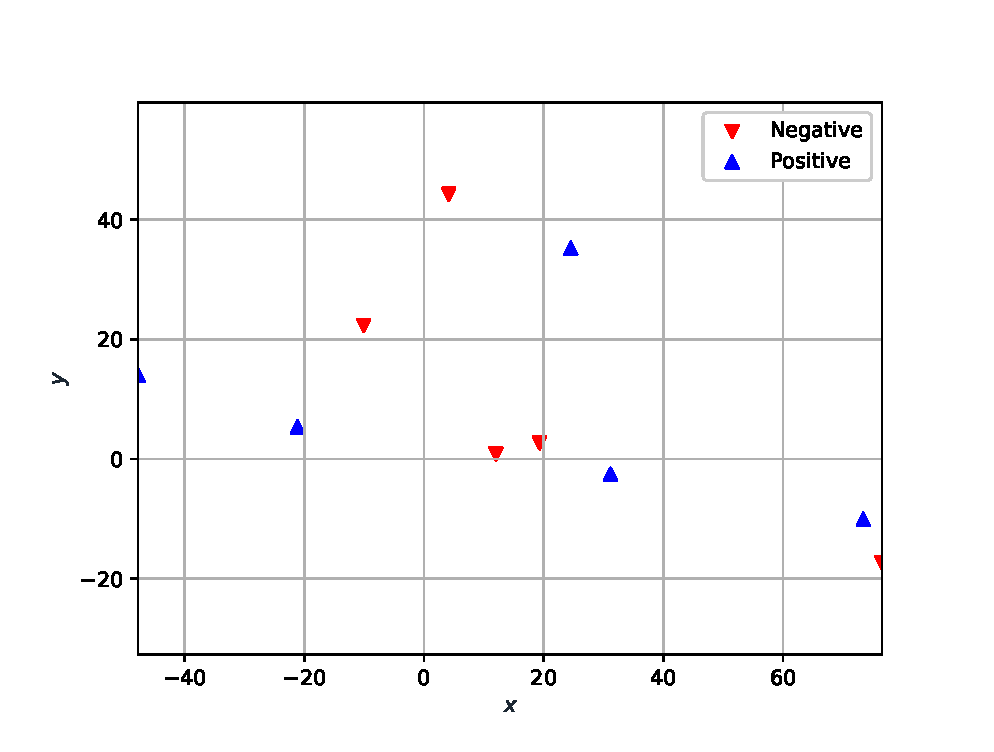
\includegraphics[scale=0.75]{figures/random}
    \caption{Calling \textit{generate\_random\_group} twice to generate 10 points }
\end{matlab}

\subsection{Linear Classification in \( \R^2 \)}

\subsubsection{Training the Linear Classifier}

Ένας γραμμικός ταξινομητής αρχικά λαμβάνει ως είσοδο ένα συνόλο αντικειμένων,
η κλάση καθενός από τα οποία είναι γνωστή εκ των προτέρων. \\

Βάσει αυτών των αντικειμένων υπολογίζονται τα \( a \in \R^{n} \) και \( b \in \R \),
όπως περιγράφηκε στην προηγούμενη ενότητα. \\

Η ακόλουθη υλοποίηση, στην οποία όλοι οι περιορισμοί,
που αναφέραμε, ενοποιούνται υπό το σύστημα \( Α \cdot x = b \),
υποθέτει κάποια εξοικείωση με τη βιβλιοθήκη \textit{SciPy} της \textit{Python}
και πιο συγκεκριμένα με τη μέθοδο
\href{https://docs.scipy.org/doc/scipy/reference/optimize.linprog-simplex.html}{linprog},
παράδειγμα χρήσης της οποίας μπορείτε να βρείτε
\href{https://stackoverflow.com/questions/45873783/python-linprog-minimization-simplex-method}{εδώ}. \\

\pagebreak

\begin{lstlisting}[caption={Calculating matrix \textbf{A} and vector \textbf{b}}]
    A = []

    for y in range(1, len(Y) + 1):

        l = [0] * (y - 1)
        r = [0] * (len(Y) + len(Z) - y)

        A.append(l + [-1] + r + [-1 * Y[y - 1][0], -1 * Y[y - 1][1], +1])

    for z in range(1, len(Z) + 1):

        l = [0] * (len(Y) + z - 1)
        r = [0] * (len(Z) - z)

        A.append(l + [-1] + r + [+1 * Z[z - 1][0], +1 * Z[z - 1][1], -1])

    for y in range(1, len(Y) + 1):

        l = [0] * (y - 1)
        r = [0] * (len(Y) + len(Z) - y)

        A.append(l + [-1] + r + [0, 0, 0])

    for z in range(1, len(Z) + 1):

        l = [0] * (len(Y) + z - 1)
        r = [0] * (len(Z) - z)

        A.append(l + [-1] + r + [0, 0, 0])

    A = np.asarray(A)

    lower, upper = [0] * (len(Y) + len(Z)), [-1] * (len(Y) + len(Z))

    b = np.asarray(upper + lower)
\end{lstlisting}

\begin{lstlisting}[caption={Defining vector \textbf{c} and finding a solution to the problem}]
    lower, upper = [0, 0, 0], [1 / len(Y)] * len(Y) + [1 / len(Z)] * len(Z)

    c = np.asarray(upper + lower)

    result = linprog(c, A_ub=A, b_ub=b, bounds=(None, None))
\end{lstlisting}

\begin{lstlisting}[caption={Determining the slope and the y-intercept of the separating line}]
    a, b, c = result.x[-3:]

    a, b = -(a / b), (c / b)
\end{lstlisting}

\begin{figure}[hp]
    \centering
    \subfloat{{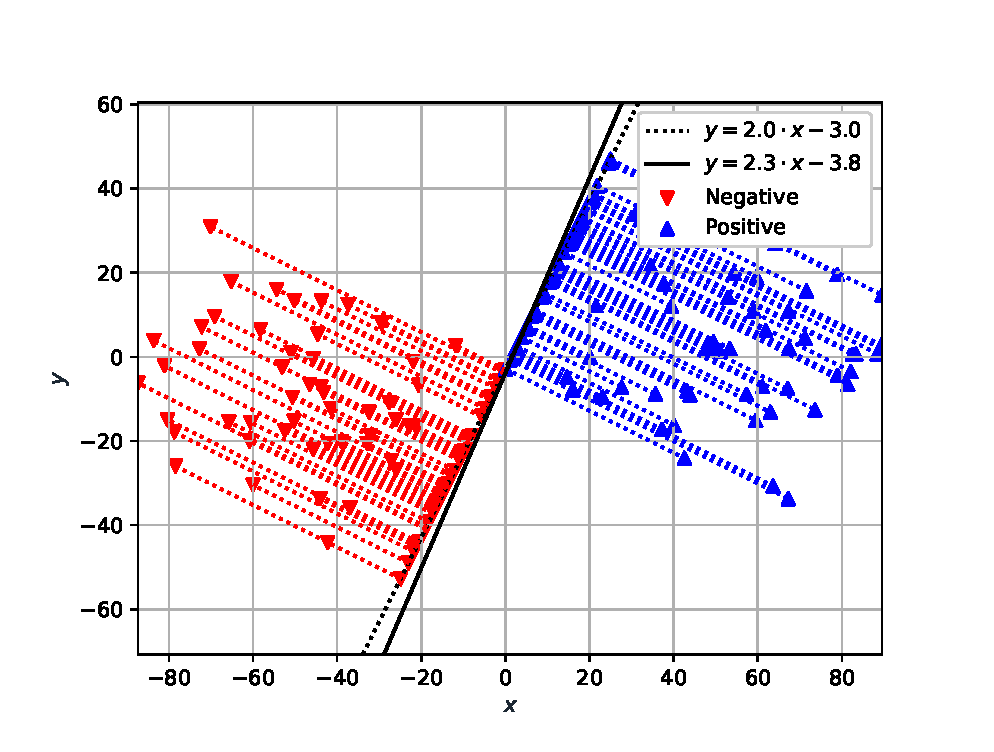
\includegraphics[width=7.5cm]{figures/linearly_separable_example_with_guides}}}
    \qquad
    \subfloat{{\includegraphics[width=7.5cm]{figures/linearly_separable_example_no_guides}}}
    \caption{Παράδειγμα επι γραμμικά διαχωρίσιμων υποσυνόλων του \( \R^2 \)}
\end{figure}

\begin{figure}[hp]
    \centering
    \subfloat{{\includegraphics[width=7.5cm]{figures/not_linearly_separable_example_no_solution}}}
    \qquad
    \subfloat{{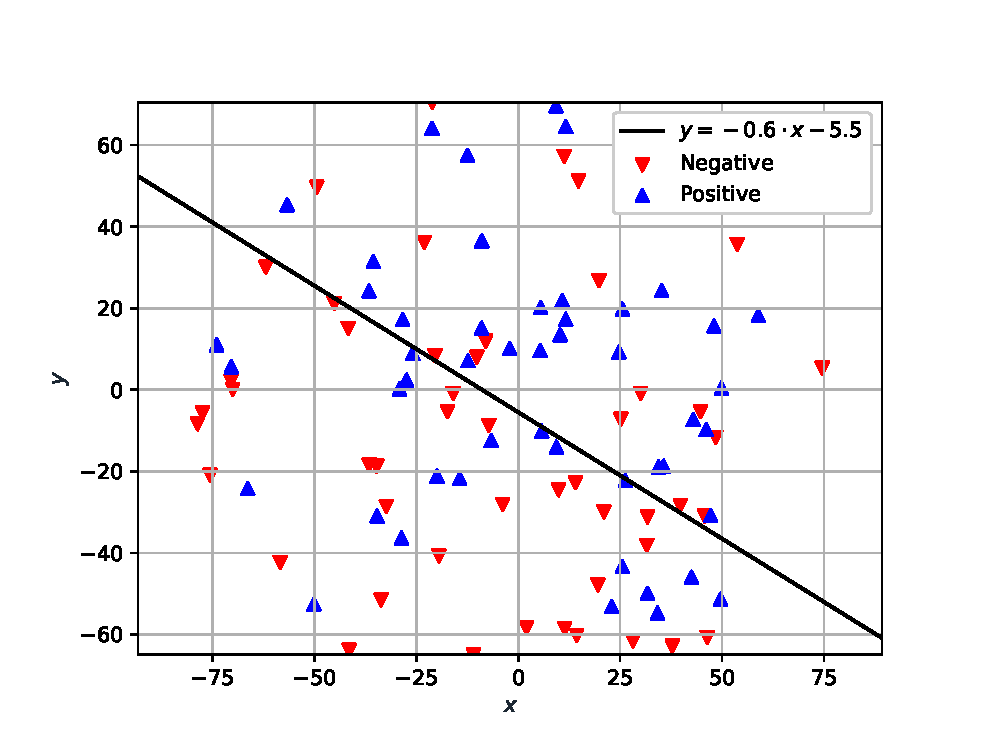
\includegraphics[width=7.5cm]{figures/not_linearly_separable_example_with_solution}}}
    \caption{Παράδειγμα επι μη γραμμικά διαχωρίσιμων υποσυνόλων του \( \R^2 \)}
\end{figure}

\subsubsection{Testing the Linear Classifier}

Χρησιμοποιούμε τυχαία στοιχεία του \( \R^2 \),
για να ελέγξουμε την ακρίβεια του γραμμικού ταξινομητή, που αναπτύξαμε. \\

Για κάθε ένα, από αυτά τα αταξινόμητα αντικείμενα, \( x \),
το πρόσημο της παράστασης \( a^{T} \cdot x - b \),
υποδεικνύει την κλάση στην οποία είναι πιθανότερο να ανήκει το αντικείμενο αυτό. \\

\begin{lstlisting}[caption={Η μέθοδος \textit{generate\_random\_points}}]
    xs, ys = [], []

    for _ in range(number):

        xs.append(random.uniform(xaxis[0], xaxis[1]))
        ys.append(random.uniform(yaxis[0], yaxis[1]))

    return xs, ys
\end{lstlisting}

\pagebreak

\begin{lstlisting}[caption={Η υλοποίηση της ταξινόμησης βάσει του προσήμου της παράστασης \( a^{T} \cdot x - b \)}]
    f = lambda x: a * x + b

    xs, ys = generate_random_points((xmin, xmax), (ymin, ymax), args.extra)

    xsa, ysa, xsb, ysb = [], [], [], []

    for i in range(len(xs)):

        if (f(xs[i]) > ys[i]) == (f(xa[0]) > 0):

            xsa.append(xs[i])
            ysa.append(ys[i])

        else:

            xsb.append(xs[i])
            ysb.append(ys[i])
\end{lstlisting}

\begin{figure}[hp]
    \centering
    \subfloat{{\includegraphics[width=7.5cm]{figures/testing_1}}}
    \qquad
    \subfloat{{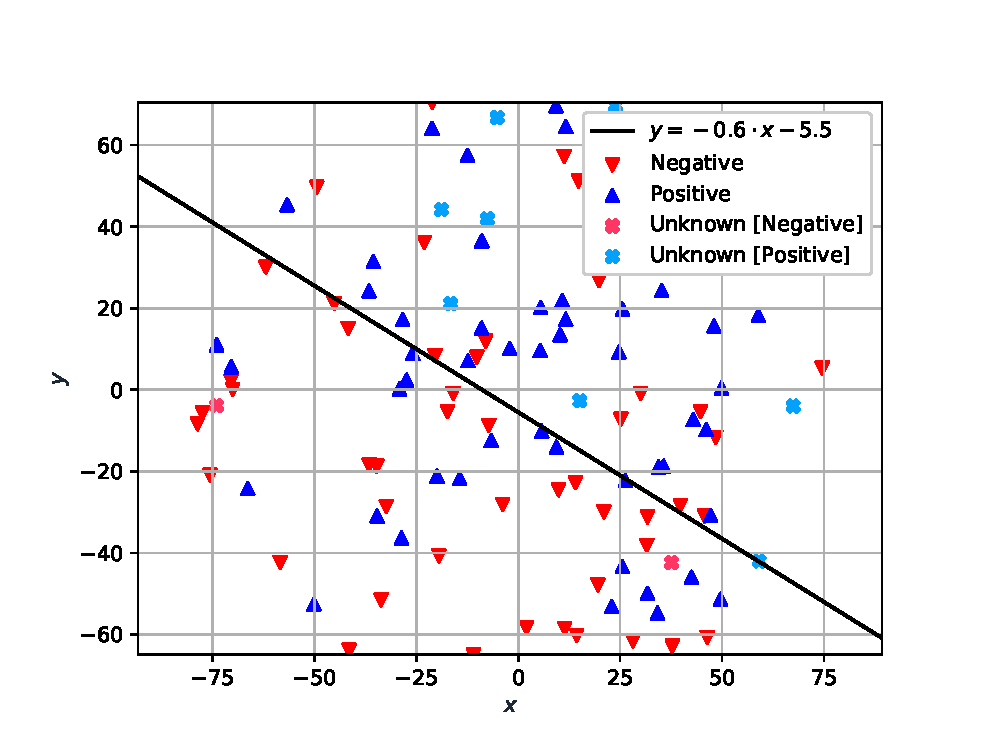
\includegraphics[width=7.5cm]{figures/testing_2}}}
    \caption{Ταξινόμηση σημείων των οποίων την κλάση δεν γνωρίζουμε εκ των προτέρων}
\end{figure}

\end{document}
